\subsection{Simulink}\label{chapter_SimulinkIMPL}

Finally, before calculating the state variable feedback factors in the next chapter, it is advisable to create a dummy state space controller in Simulink. Therefore it is necessary to know what the actuating variables are. Figure \ref{fig:Remote control stimuli} shows these input variables named \textit{phi\_set}, \textit{theta\_set}, \textit{rpsi\_set} and \textit{thrust\_set}. The thrust is controlled directly by the remote control and does not have to be controlled in the quadrocopter. The other three variables are the set variables that must be controlled internal. \\
In addition the input of the process - thus the output of the controller - has to be defined. As figure \ref{fig:Controller block} shows, the outputs of the controller block are the desired pseudo forces for the four motors of the quadrocopter.

The three set variables calculated by the controller and the thrust are mixed together and four pseudo forces are the result. This is very easy to understand - for example \textit{phi\_set} tells, that the quadrocopter shall move to the left, so the left motor is slowed down and the right one is accelerated. 

\begin{figure}
	\centering
		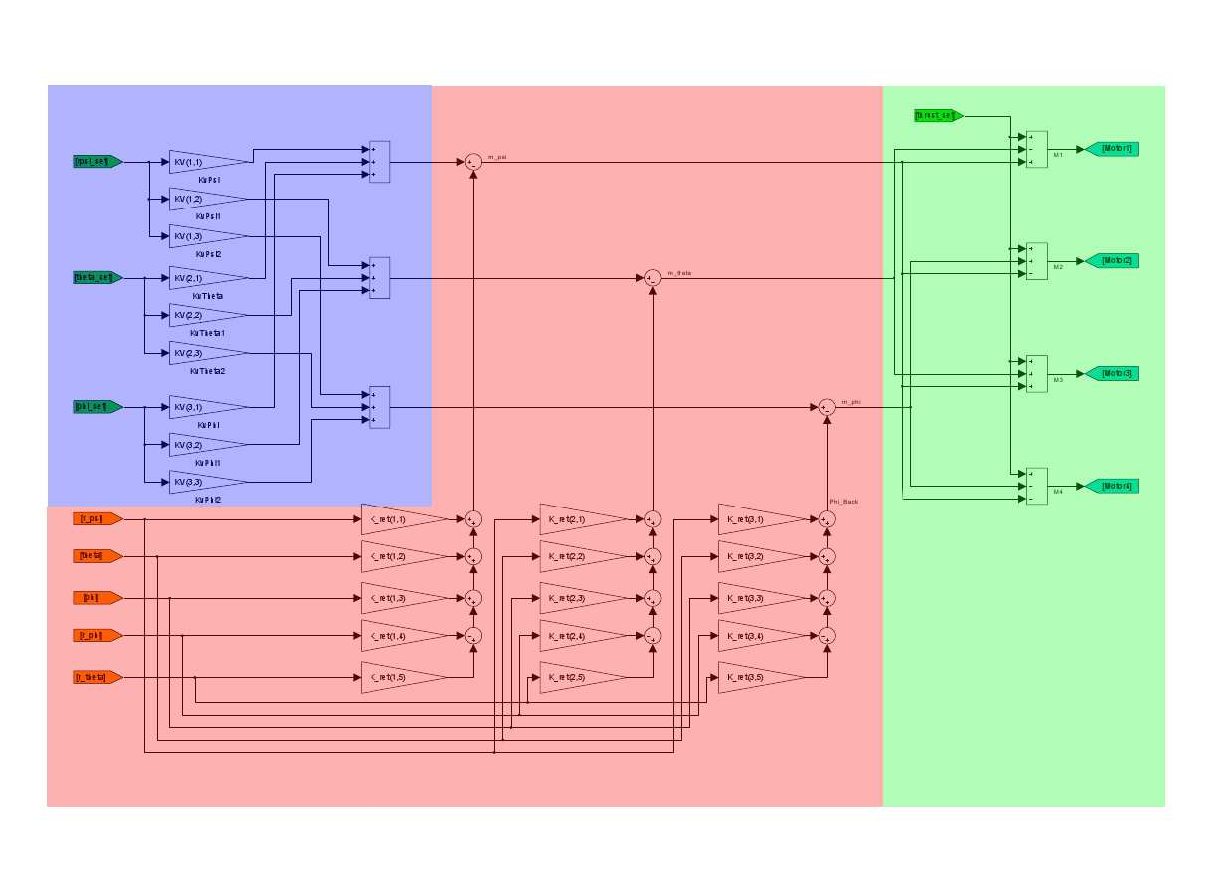
\includegraphics[width=1.00\textwidth]{03_Grafiken/SS_overview.pdf}
	\caption{Overview over the whole state space controller}
	\label{fig:SS_overview}
\end{figure}

Figure \ref{fig:SS_overview} shows the complete state space controller. In the following sub chapters the red and blue part are explained. 

\begin{figure}
	\centering
		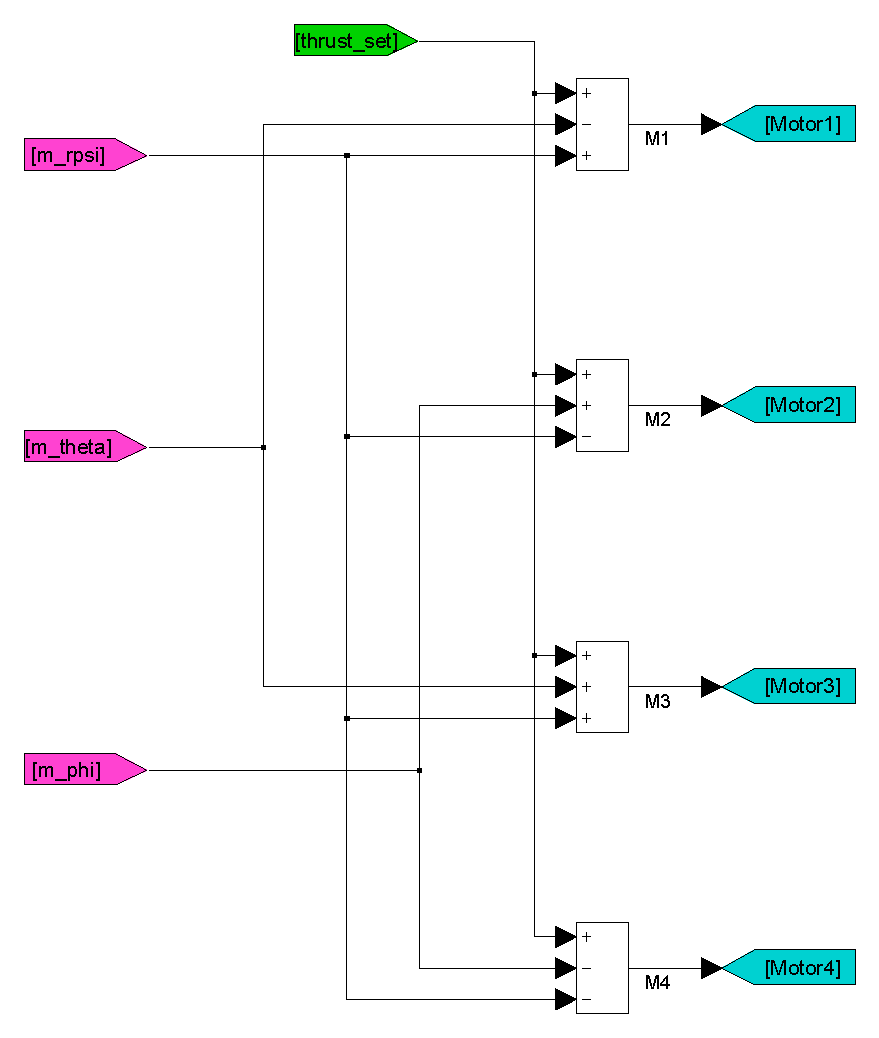
\includegraphics[width=0.60\textwidth]{03_Grafiken/SS_Trafo.pdf}
	\caption{Transformation of the set values to pseudo forces}
	\label{fig:SS_Trafo}
\end{figure}

Figure \ref{fig:SS_Trafo} shows this green part in detail. This part is something like a transformation from set values, for every moving direction of the quadrocopter, to pseudo forces. Giving more \textit{thrust}, all four motors are accelerated and the result is, that the quadrocopter raises. Changing \textit{m\_rpsi} means, accelerating two motors and decelerating the other two. In this case, the quadrocopter is yawing. For \textit{m\_theta} and \textit{m\_phi} it is both nearly the same. One motor is accelerated and the opposing motor is decelerated. The quadrocopter flies in direction of the decelerated motor. \\
For sure, all combinations of these four input values are possible. 